\section{Estado del arte}

% OSNT
\begin{frame}{The Open Source Network Tester}
  \begin{itemize}
    \item Sistema de captura y reproducción de código abierto
    \item Utiliza una FPGA del mismo modelo que este TFG
    \item Gestionada desde una interfaz sobre el propio servidor
    \item Aspectos mejorables
    \begin{itemize}
      \item Provee información exlusivamente de la FPGA
      \item Rendimiento puede estar limitado por la velocidad del disco
      \begin{itemize}
        \item No alerta al usuario de ello
      \end{itemize}
      \item Se maneja desde el propio servidor
      \begin{itemize}
        \item No es accesible por terceros sin ceder el uso completo de la máquina
        \item Problema si se satura y la interfaz deja de responder
      \end{itemize}
      \item No resuelve la conversión entre formatos de trazas
    \end{itemize}
  \end{itemize}
\end{frame}

% OSNT - Interfaz
\begin{frame}{The Open Source Network Tester - Interfaz}
  \begin{figure}
    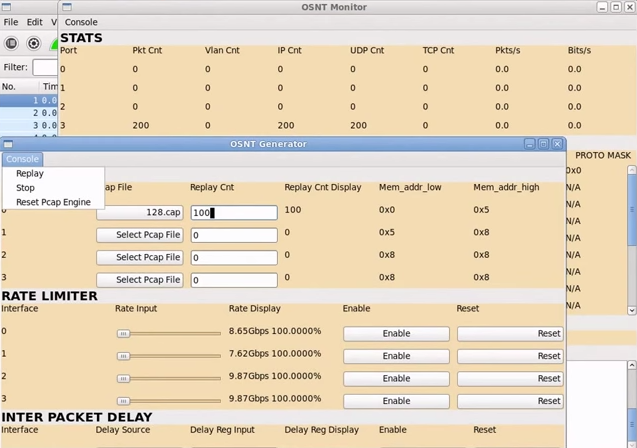
\includegraphics[width=0.9\linewidth]{osnt}
  \end{figure}
\end{frame}
